\documentclass[border=15pt]{standalone}
\usepackage{tikz,amsmath}
\usetikzlibrary{arrows.meta}

% ========== 配色 ==========
\definecolor{hid}{RGB}{52,58,143}
\definecolor{in}{RGB}{32,102,32}
\definecolor{ye}{RGB}{180,150,20}
\definecolor{or}{RGB}{190,110,20}
\definecolor{out}{RGB}{143,52,52}
\definecolor{hidFill}{RGB}{199,203,243}
\definecolor{inFill}{RGB}{183,224,177}
\definecolor{yeFill}{RGB}{252,240,180}
\definecolor{orFill}{RGB}{250,224,180}
\definecolor{outFill}{RGB}{243,199,199}

\begin{document}
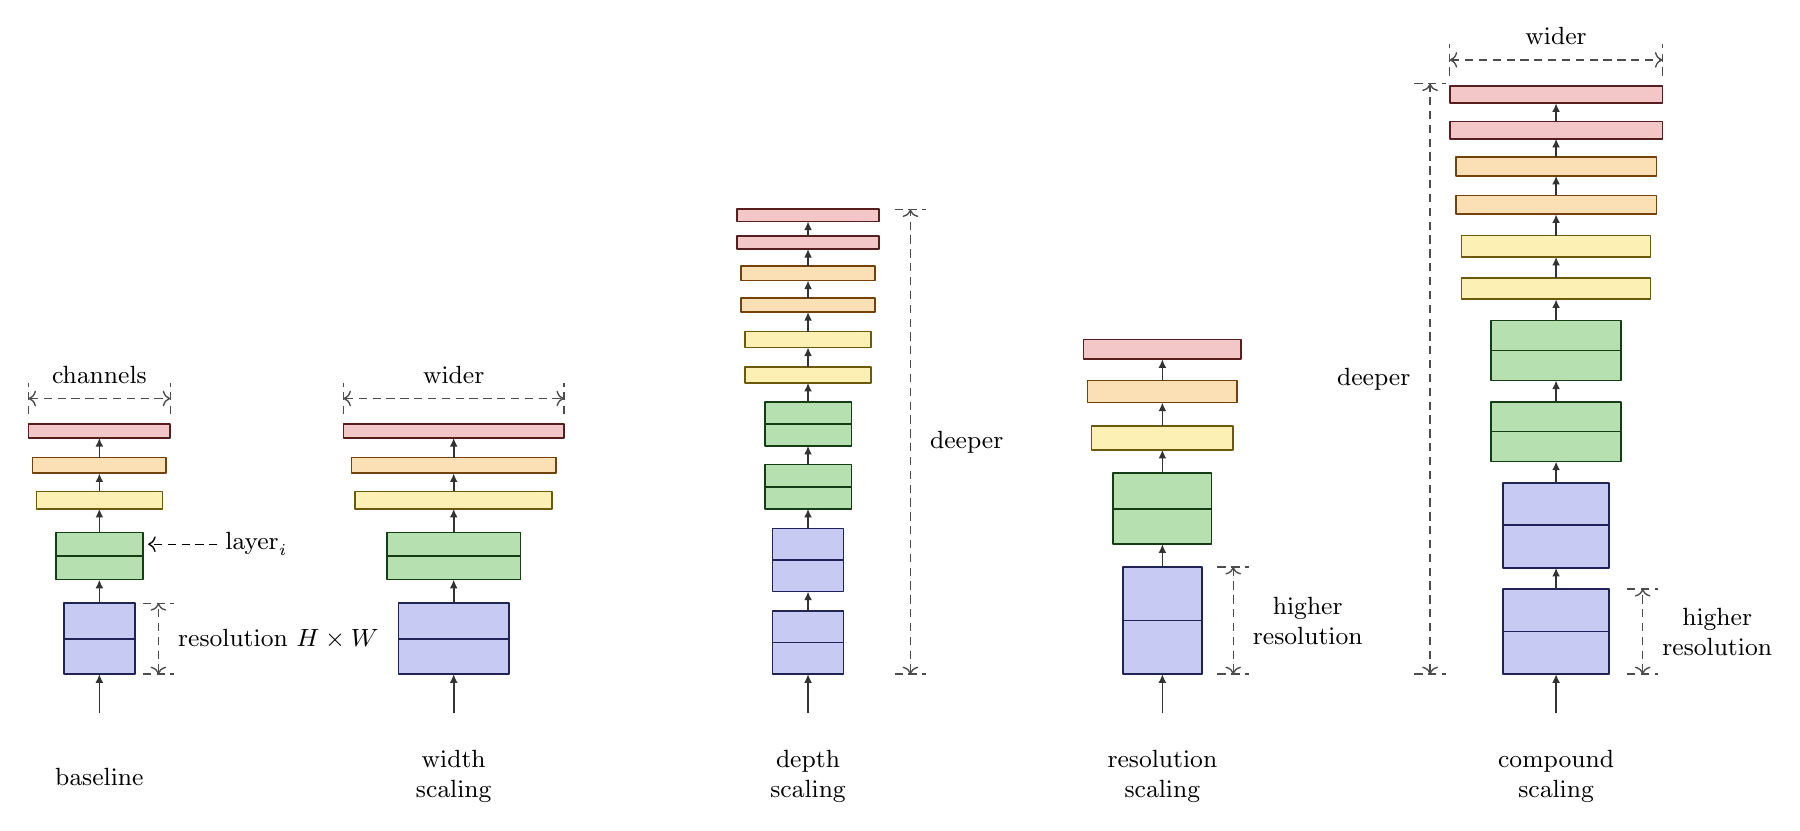
\begin{tikzpicture}[
    font=\small, line join=round,
    every node/.style={inner sep=0pt, outer sep=0pt, align=center},
    up/.style={-{Latex[length=1.1mm, width=1mm]}, line width=.6pt, black!80},
    ms/.style={<->, densely dashed, line width=.5pt, black!70}
  ]

  % ========== 宏 ==========
  \newcommand{\barr}[5]{%
    \fill[#5Fill, draw=#5!60!black, line width=.6pt] ({#1-#3/2},#2) rectangle ++(#3,#4);
  }
  \newcommand{\uparr}[3]{\draw[up] (#1,#2) -- (#1,#3);}
  \newcommand{\hmeasure}[4]{%
    \draw[ms] (#1,#3) -- (#2,#3);
    \draw[densely dashed, line width=.5pt, black!70] (#1,{#3-.2})--(#1,{#3+.2}) (#2,{#3-.2})--(#2,{#3+.2});
    \node at ({(#1+#2)/2},{#3+.3}) {#4};
  }
  \newcommand{\vmeasure}[4]{%
    \draw[ms] (#1,#2) -- (#1,#3);
    \draw[densely dashed, line width=.5pt, black!70] ({#1-.2},#2)--({#1+.2},#2) ({#1-.2},#3)--({#1+.2},#3);
    \node[anchor=west] at ({#1+.25},{(#2+#3)/2}) {#4};
  }
  \newcommand{\vmeasureL}[4]{%
    \draw[ms] (#1,#2) -- (#1,#3);
    \draw[densely dashed, line width=.5pt, black!70] ({#1-.2},#2)--({#1+.2},#2) ({#1-.2},#3)--({#1+.2},#3);
    \node[anchor=east] at ({#1-.25},{(#2+#3)/2}) {#4};
  }

  % ================= baseline =================
  \uparr{2}{-.3}{.2}
  \barr{2}{.2}{.9}{.45}{hid}\barr{2}{.65}{.9}{.45}{hid}
  \uparr{2}{1.1}{1.4}
  \barr{2}{1.4}{1.1}{.3}{in}\barr{2}{1.7}{1.1}{.3}{in}
  \uparr{2}{2.0}{2.3}
  \barr{2}{2.3}{1.6}{.22}{ye}
  \uparr{2}{2.52}{2.75}
  \barr{2}{2.75}{1.7}{.2}{or}
  \uparr{2}{2.95}{3.2}
  \barr{2}{3.2}{1.8}{.18}{out}
  \hmeasure{1.1}{2.9}{3.7}{channels}
  \draw[->, densely dashed, line width=.5pt] (3.5,1.85) -- (2.62,1.85);
  \node[anchor=west] at (3.6,1.85) {$\text{layer}_{i}$};
  \vmeasure{2.75}{.2}{1.1}{resolution $H\times W$}
  \node at (2,-1.1) {baseline};

  % ================= width scaling =================
  \uparr{6.5}{-.3}{.2}
  \barr{6.5}{.2}{1.4}{.45}{hid}\barr{6.5}{.65}{1.4}{.45}{hid}
  \uparr{6.5}{1.1}{1.4}
  \barr{6.5}{1.4}{1.7}{.3}{in}\barr{6.5}{1.7}{1.7}{.3}{in}
  \uparr{6.5}{2.0}{2.3}
  \barr{6.5}{2.3}{2.5}{.22}{ye}
  \uparr{6.5}{2.52}{2.75}
  \barr{6.5}{2.75}{2.6}{.2}{or}
  \uparr{6.5}{2.95}{3.2}
  \barr{6.5}{3.2}{2.8}{.18}{out}
  \hmeasure{5.1}{7.9}{3.7}{wider}
  \node at (6.5,-1.1) {width\\scaling};

  % ================= depth scaling =================
  \uparr{11}{-.3}{.2}
  \barr{11}{.2}{.9}{.4}{hid}\barr{11}{.6}{.9}{.4}{hid}
  \uparr{11}{1.0}{1.25}
  \barr{11}{1.25}{.9}{.4}{hid}\barr{11}{1.65}{.9}{.4}{hid}
  \uparr{11}{2.05}{2.3}
  \barr{11}{2.3}{1.1}{.28}{in}\barr{11}{2.58}{1.1}{.28}{in}
  \uparr{11}{2.86}{3.1}
  \barr{11}{3.1}{1.1}{.28}{in}\barr{11}{3.38}{1.1}{.28}{in}
  \uparr{11}{3.66}{3.9}
  \barr{11}{3.9}{1.6}{.2}{ye}
  \uparr{11}{4.1}{4.35}
  \barr{11}{4.35}{1.6}{.2}{ye}
  \uparr{11}{4.55}{4.8}
  \barr{11}{4.8}{1.7}{.18}{or}
  \uparr{11}{4.98}{5.2}
  \barr{11}{5.2}{1.7}{.18}{or}
  \uparr{11}{5.38}{5.6}
  \barr{11}{5.6}{1.8}{.16}{out}
  \uparr{11}{5.76}{5.95}
  \barr{11}{5.95}{1.8}{.16}{out}
  \vmeasure{12.3}{.2}{6.1}{deeper}
  \node at (11,-1.1) {depth\\scaling};

  % ================= resolution scaling =================
  \uparr{15.5}{-.3}{.2}
  \barr{15.5}{.2}{1.0}{.68}{hid}\barr{15.5}{.88}{1.0}{.68}{hid}
  \uparr{15.5}{1.56}{1.85}
  \barr{15.5}{1.85}{1.25}{.45}{in}\barr{15.5}{2.3}{1.25}{.45}{in}
  \uparr{15.5}{2.75}{3.05}
  \barr{15.5}{3.05}{1.8}{.3}{ye}
  \uparr{15.5}{3.35}{3.65}
  \barr{15.5}{3.65}{1.9}{.28}{or}
  \uparr{15.5}{3.93}{4.2}
  \barr{15.5}{4.2}{2.0}{.25}{out}
  \vmeasure{16.4}{.2}{1.56}{higher\\resolution}
  \node at (15.5,-1.1) {resolution\\scaling};

  % ================= compound scaling =================
  \uparr{20.5}{-.3}{.2}
  \barr{20.5}{.2}{1.35}{.54}{hid}\barr{20.5}{.74}{1.35}{.54}{hid}
  \uparr{20.5}{1.28}{1.55}
  \barr{20.5}{1.55}{1.35}{.54}{hid}\barr{20.5}{2.09}{1.35}{.54}{hid}
  \uparr{20.5}{2.63}{2.9}
  \barr{20.5}{2.9}{1.65}{.38}{in}\barr{20.5}{3.28}{1.65}{.38}{in}
  \uparr{20.5}{3.66}{3.93}
  \barr{20.5}{3.93}{1.65}{.38}{in}\barr{20.5}{4.31}{1.65}{.38}{in}
  \uparr{20.5}{4.69}{4.96}
  \barr{20.5}{4.96}{2.4}{.27}{ye}
  \uparr{20.5}{5.23}{5.5}
  \barr{20.5}{5.5}{2.4}{.27}{ye}
  \uparr{20.5}{5.77}{6.04}
  \barr{20.5}{6.04}{2.55}{.24}{or}
  \uparr{20.5}{6.28}{6.53}
  \barr{20.5}{6.53}{2.55}{.24}{or}
  \uparr{20.5}{6.77}{7.0}
  \barr{20.5}{7.0}{2.7}{.22}{out}
  \uparr{20.5}{7.22}{7.45}
  \barr{20.5}{7.45}{2.7}{.22}{out}
  \hmeasure{19.15}{21.85}{8.0}{wider}
  \vmeasureL{18.9}{.2}{7.7}{deeper}
  \vmeasure{21.6}{.2}{1.28}{higher\\resolution}
  \node at (20.5,-1.1) {compound\\scaling};

\end{tikzpicture}
\end{document}